\chapter[Cryo-EM and SPA]{Cryo-electron microscopy and single particle analysis}\label{em}

Knowing the structure of macromolecular complexes is often crucial to understand --- and potentially take control of --- the function and behavior of biological systems.
To this end, structural biologists employ several techinques to unveil the structure of biomolecules and their complexes: typically proteins, nucleic acids and their ligands.

Arguably, the three giants in the field are X-ray crystallography, Nuclear Magnetic Resonance (NMR) and cryo-electron microscopy (cryo-EM), with several other techniques playing complementary, more specialized or niche roles (such as mass spectroscopy, neutron scattering or small-angle scattering).
In recent years, machine-learning (ML) structure prediction tools such as AlphaFold~\cite{jumperHighlyAccurateProtein2021,abramsonAccurateStructurePrediction2024} and RoseTTAFold~\cite{baekAccuratePredictionProtein2021} have also conquered their way into the forefront of structural biology techniques, computationally predicting protein structures with unprecedented precision and without the wait and costs of experimental approaches.
Each technique has pros and cons, making it suited to different samples and applications.

In X-ray crystallography --- in many ways the predecessor to cryo-EM as the all-purpose structural biology technique --- crystals are grown from the sample of interest; the crystals are then illuminated by an X-ray beam, and the diffraction pattern thus created can be detected and used to reconstruct the three-dimensional (3D) structure of the sample.
Thanks to the short wavelength of X-rays --- as opposed to visible light --- it is possible to localize the positions of atoms with sub-angstrom precision.
X-ray crystallography has played a major role in the development of structural biology, and is still the primary source of protein structures on the Protein Data Bank~\cite{bermanProteinDataBank2000,bermanAnnouncingWorldwideProtein2003}.
However, the need for crystallization constitutes a major bottleneck: it requires very pure and homogeneous samples, and the procedure is often hard to devise and reproduce, requiring time, resources and some luck.
Moreover, the protein is forced into a specific crystalline lattice, restricting the conformational freedom of the molecule and potentially limiting the biological significance of the obtained structures~\cite{ravikumarComparisonSidechainDispersion2022}.

% TODO: somewhere here mention like covid spikes to show how important structures are?

\localtableofcontents

\section{Cryo-EM: basic concepts}

Cryo-EM improves on these aspects by forgoing crystallization in favor of sample vitrification, which allows to capture the sample in a near-native state. This requires analysing many individual particles in different orientations, in a procedure known as single particle analysis (SPA).

In simple terms, the electron microscope works by shooting a coherent electron beam at the sample, and using a camera to detect the scattered electrons and form an image.
Thanks to the small wavelength of electrons, cryo-EM can reach much higher resolution than light microscopy.
In the last decade, the development of direct electron detectors made it possible to reach atomic resolutions, jump-starting to the so-called resolution revolution and the rise of cryo-EM as one of the primary methods for high resolution structure determination~\cite{faruqiCCDDetectorsHighresolution2000}.

Instead of relying on amplitude contrast for image formation, transmission electron microscopy uses phase contrast, which is caused by elastic scattering events affecting the electrons traversing the sample.
Some electrons, however, are inelastically scattered; these electrons are no longer coherent, and therefore add to the noise of the image.
Increasing the electron dose can help improve the signal-to-noise ratio (SNR), but comes at the cost of radiation damage, which denatures the sample and rapidly destroys high-resolution information.
For these reasons, a significant limitation --- and thus optimization target --- of cryo-EM is the low SNR.

The cryo-EM workflow is well established, and usually consists of the same principal components: sample preparation and vitrification, data collection, preprocessing (cleaning, motion and CTF correction), particle picking and classification, three-dimensional (3D) reconstruction, and model building.
This section describes such typical workflow, expanding on the theoretical bases underlying each step.

\begin{figure}[ht]
    \centering
    \includegraphics[width=.5\textwidth]{example-image.png}
    \titledcaption[Cryo-EM workflow]{TODO: typical cryoem workflow}
    \label{fig:em_workflow}
\end{figure}

\section{Sample preparation}
Cryo-EM samples for SPA are usually prepared in vitro by expressing ad purifying the protein or complex of interest to create a minimal system.
Sample concentration and purity are important variables to control, as they will affect vitrification and data processing complexity.
The sample solution is then deposited on a cryo-EM grid and vitrified via plunge freezing in liquid ethane or other methods (\autoref{fig:em_plunge_freezing})~\cite{dubochetCryoelectronMicroscopyVitrified1988}.
Vitrification allows to fix the sample in near-native, hydrated conditions while avoiding the formation of crystalline ice, which would damage the sample.
When vitrifying, the thickness of the ice is crucial: a thinner layer will result in fewer inelastically scattered electrons during data collection and better SNR.
However, too-thin ice can crack and increase issues with preferential orientation or particle distribution.

\begin{figure}[ht]
    \centering
    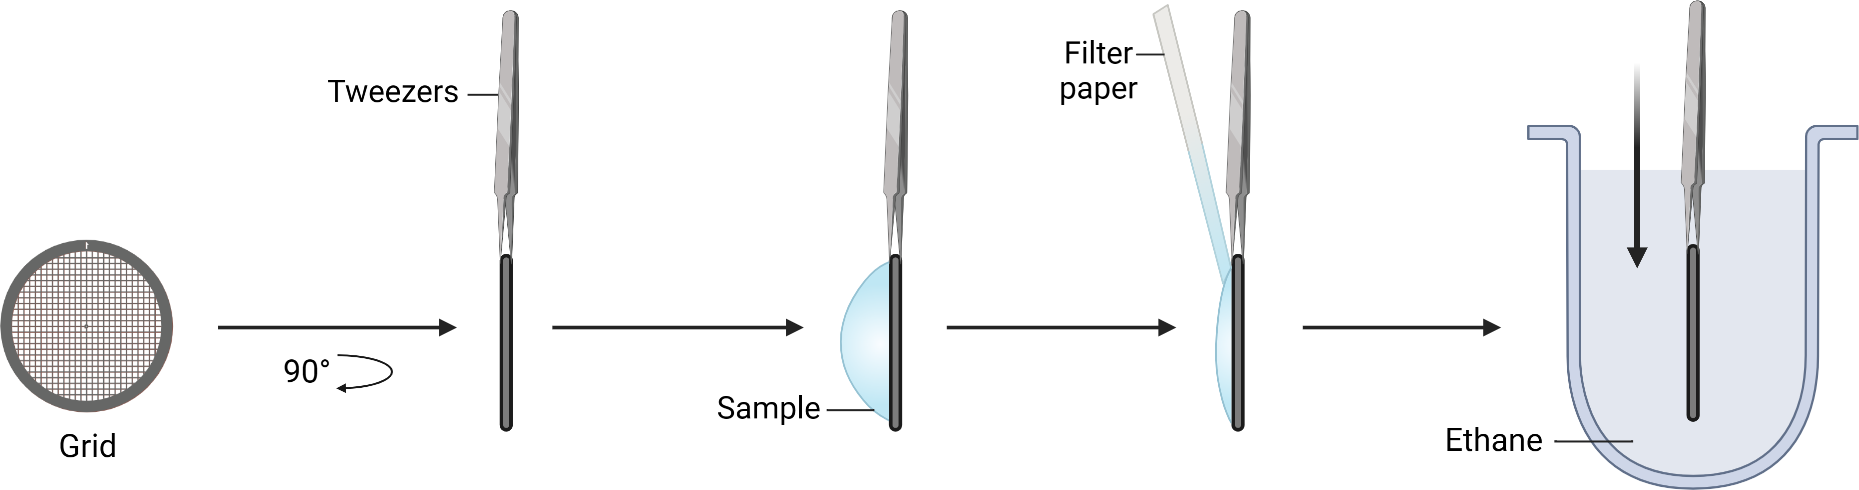
\includegraphics[width=\textwidth]{introduction/plunge_freezing.png}
    \titledcaption[Vitrification via plunge freezing]{Typical vitrification procedure via plunge freezing. A drop of sample is placed on the grid, blotted with a filter paper to reduce its thickness to a thin layer, and then plunged into liquid ethane. Figure adapted from \citet{chungNobelPrizeChemistry2017}.}
    \label{fig:em_plunge_freezing}
\end{figure}

Novel approaches are beginning to use jets, sprays and microfluidics in order to obtain uniform, thin and more rapidly vitrified samples~\cite{geminEasyGridVersatilePlatform2024}.

\subsection{Preferential orientation}\label{em_pref_ori}
A common issue with sample preparation for cryo-EM is non-uniform orientation distribution of the protein in the vitrified sample, often due to particles being adsorbed to the air-water interface~\cite{nobleRoutineSingleParticle2018}.

Strong preferential orientation may completely preclude the ability to do a 3D reconstruction, due to the lack of a wide distribution of orientations (\fullref{em_reconstruction}).
When this problem arises, there are a few ways to tackle it during sample preparation.
The most common is the addition of small amounts of detergents to occupy the air-water interface and prevent particles from preferentially orienting hydrophobic surfaces out of the water.
Other methods are a bit more involved, such as the use of functionalized graphene grids~\cite{luFunctionalizedGrapheneGrids2022}, streptavidin-coated affinity support grids~\cite{crucifixImmobilizationBiotinylatedDNA2004,hanLongShelflifeStreptavidin2016}, but can offer more control over the orientation of the particles in the sample.

Alternatively, preferential orientation can be partially dealt with by collecting a tilted dataset, effectively forcing the target object into a different orientation.
This method comes at the cost of worse SNR due to the thicker sample, increased motion due to doming, and worse CTF estimation.
However, it was recently shown that the effect of these issues on the final resolution can be rendered negligible with careful preprocessing~\cite{aiyerOvercomingResolutionAttenuation2024}.

\section{Data collection}
The vitrified sample is loaded into the electron microscope (under cryogenic conditions and vacuum, in order to maintain the sample vitrified and uncontaminated), and suitable positions on the grid are chosen for imaging, prioritizing for: presence of the target protein or complex, fewer contaminations, and lower ice thickness.
In modern workflows and software, this step and the subsequent data collection are increasingly automated, allowing for higher throughput (up to a dozen-thousand images per day) and lower human intervention~\cite{schorbSoftwareToolsAutomated2019}.

During collection, the sample stage and/or electron beam are moved to each position to collect micrographs.
At each position, a short movie is recorded, consisting of a few low-dose, short-exposure frames: this allows to reduce the blur caused by intra-frame motion (induced by external factors among which the electron beam itself); the frames will later be aligned and averaged to produce a single higher-contrast image.
Direct detectors are therefore crucial not only for their raw improvement in achievable resolution, but also for their high speed, contributing to the reduction of yet another source of noise.

An important concept to be mindful of when setting up a data collection is defocus; in order to better understand how defocus affects later processing steps, we first need to understand image formation in the electron microscope, and the importance of estimating and correcting the Contrast Transfer Function (CTF).

\subsection{Image formation}

In electron microscopy, image contrast derives almost entirely from phase contrast.
The electron beam generated by the microscope is initially coherent, that is the phases of all the electrons in the beam are correlated.
When electrons traverse the sample, they have a chance to undergo elastic scattering by the sample nuclei; this results in a shift in the electron's phase, leading to interference with the unscattered wave at the image plane (\autoref{fig:em_image_formation}).
It's this interference that creates phase contrast, which the camera detects to generate the image.
Because the fraction of scattered electrons is very low, the resulting beam has nearly the same amplitude as the non scattered beam, resulting in low contrast images.

Some electrons are also inelastically scattered by the electron clouds of the sample: these electrons lose energy and coherence, and are therefore adding to the noise of the image because the lenses no longer focus them to the right place.
To mitigate this effect, inelastically scattered electrons are filtered out using an energy filter, which removes electrons with energy that differs significantly from the unscattered ones (\autoref{fig:em_image_formation}).

Inelastic scattering is also the source of radiation damage: the energy lost by these electrons is transferred to the sample, denaturing and deforming it and thus affecting SRN.

Sample thickness is of crucial importance for image formation: higher thickness results in higher chance for collision, increasing the chance of inelastic scatterings.
Additionally, a thicker sample may result in multiple elastic scattering events, which further alter the phase but cannot be distinguished from single scattering events, contributing to image noise.

\begin{figure}[ht]
    \centering
    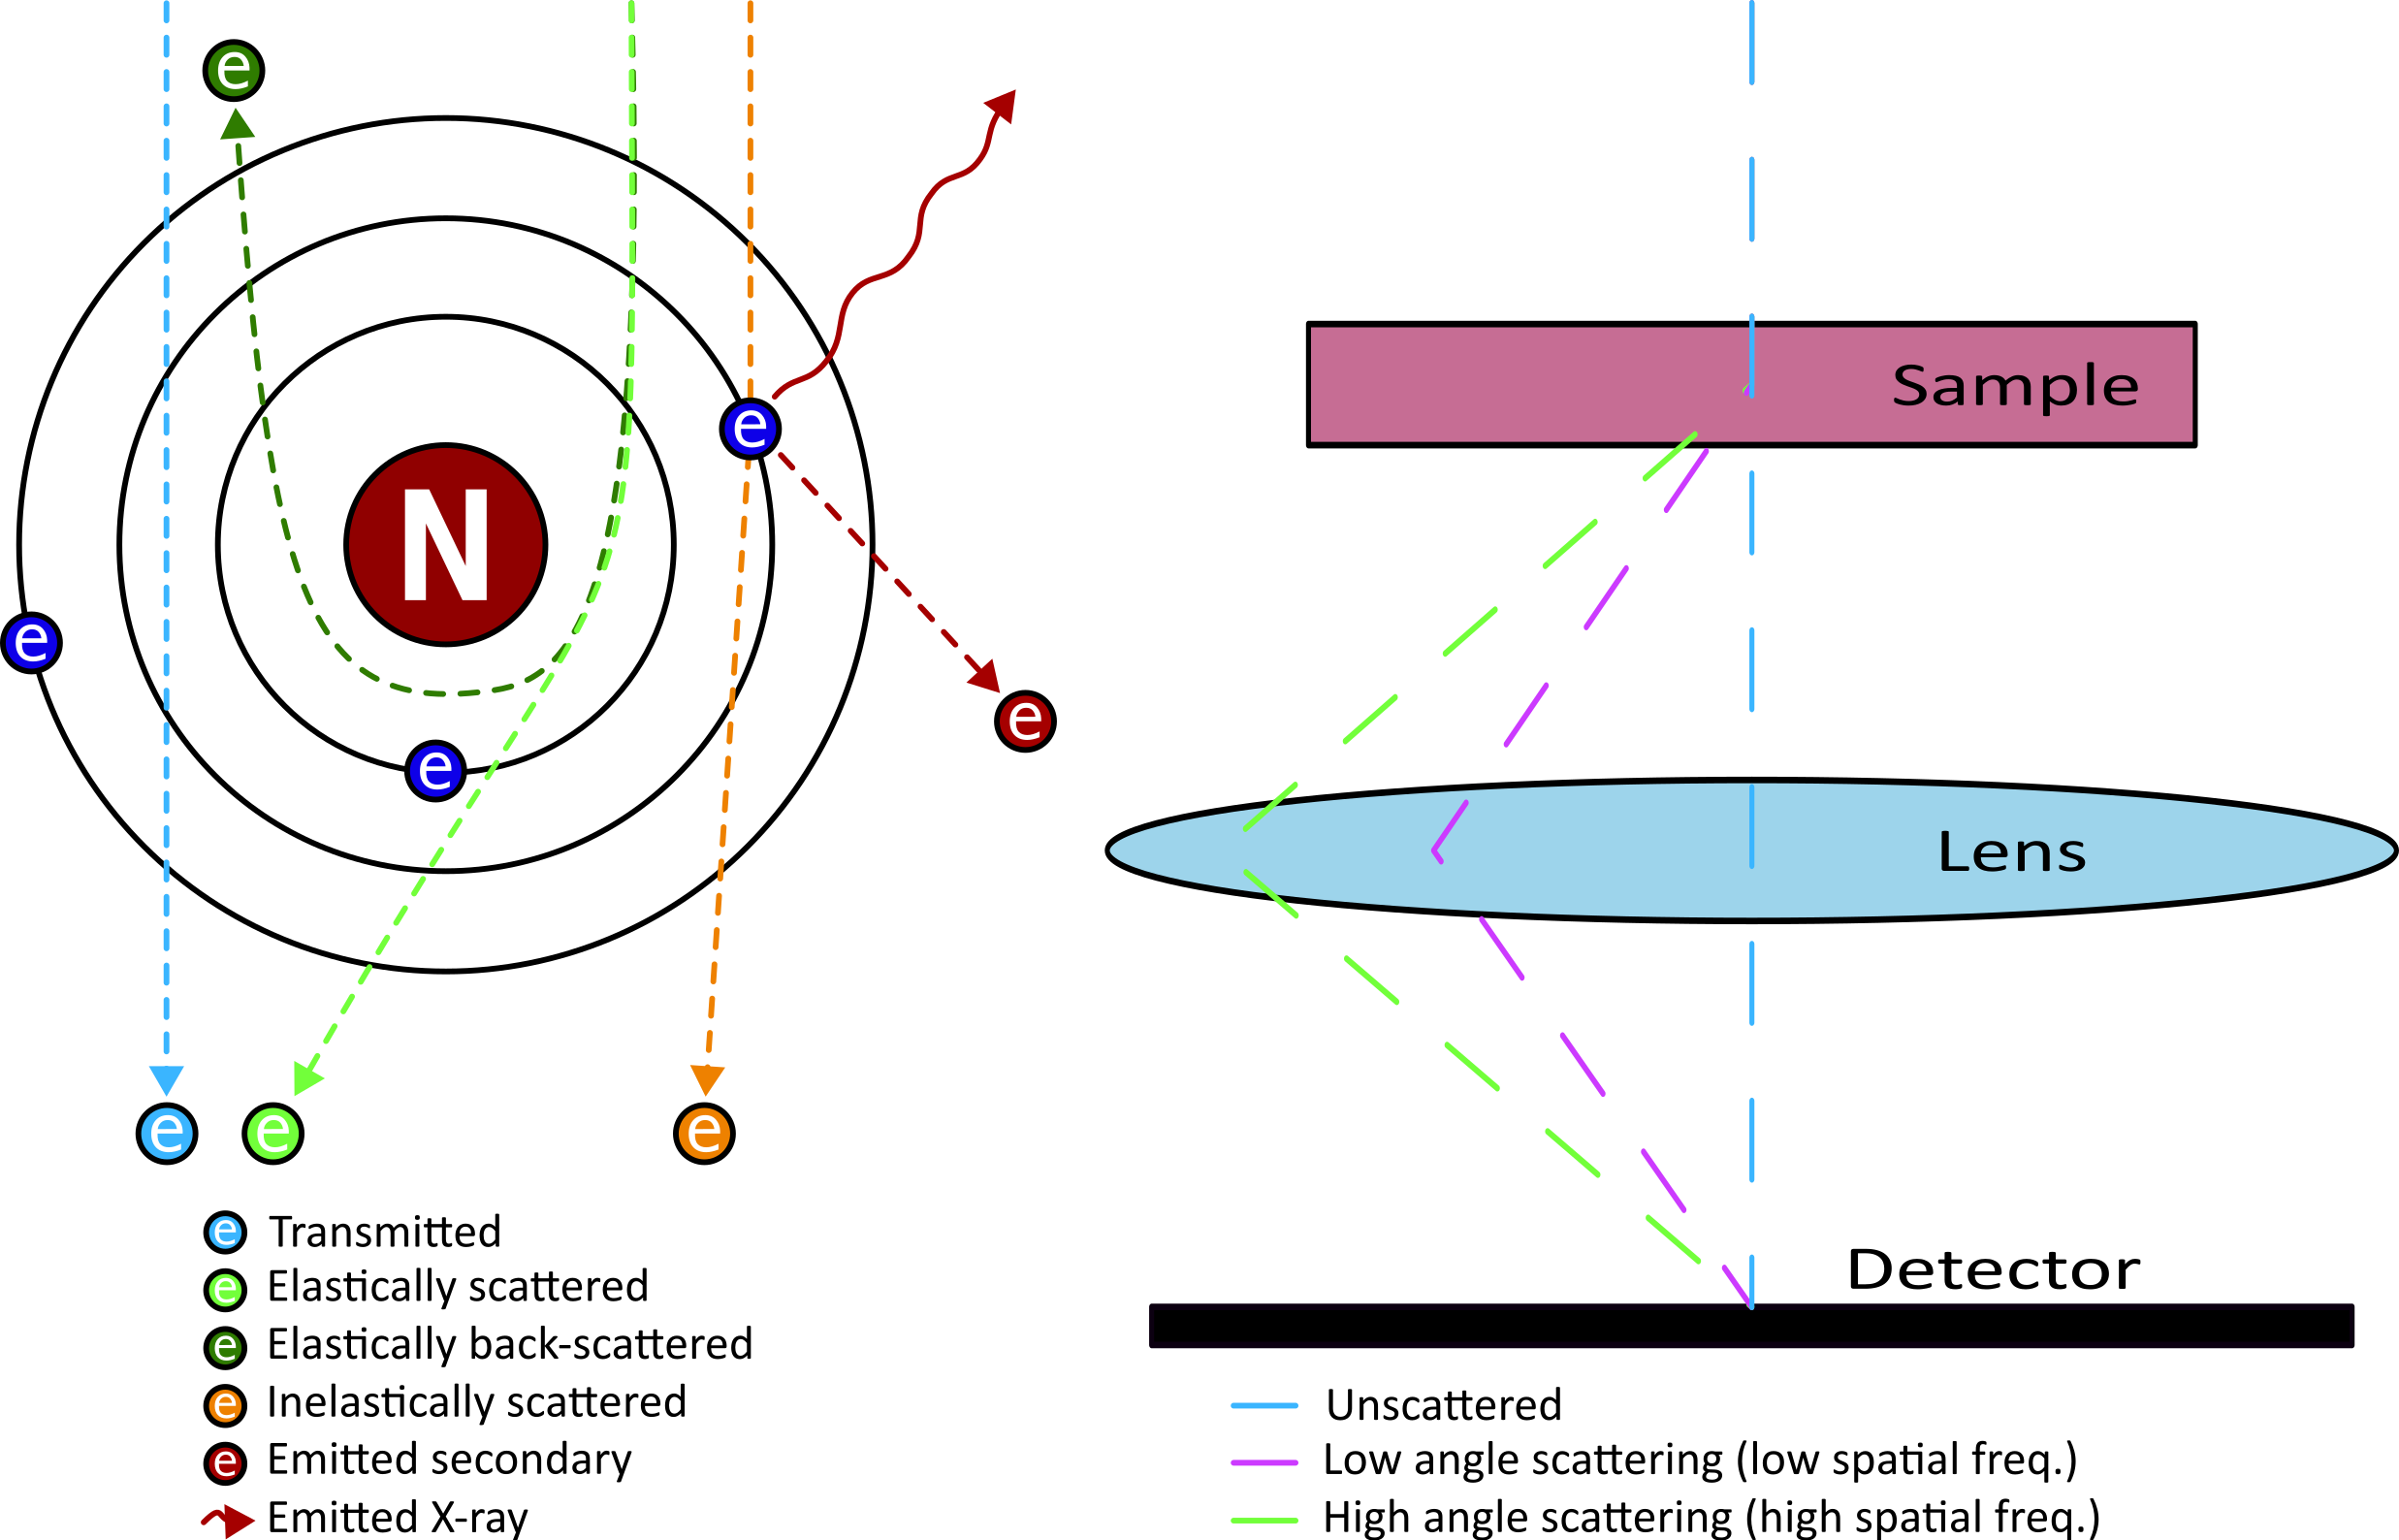
\includegraphics[width=\textwidth]{introduction/scattering.png}
    \titledcaption[Image formation]{Electron scattering and diffraction are the physical processes at the core of cryo-EM image formation. Electrons can scatter in several different ways (left), but only elastic scattering contributes to image formation via phase contrast with the trasmitted electrons. Features contained in the sample that present different spatial frequencies result in scattering at different angles (right); depending on the difference in path travelled and the wavelength of the electron beam, this results in interference between differently scattered waves. In this figure where wave oscillations are visualized as dashed lines, we can see that the unscattered and low-angle scattered waves result in constructive interference, while the high-angle scattered waves interfere destructively.}
    \label{fig:em_image_formation}
\end{figure}

\subsection{Contrast Transfer Function}\label{em_ctf}
The shift induced in the phase of the electron wave by elastic scattering events is closely related to the spatial frequency of features in the sample: smaller details such as the relative positioning of neighboring \alpha-helices, which contain information at higher spatial frequency, will scatter to higher angles; bigger features such as biological membranes will scatter to lower angles.
Depending on the angle, the interference at the image plane will be constructive or destructive, resulting in certain spatial frequencies being dampened or lost.

The CTF is a function that describes exactly this: how signal is transmitted through the sample and onto the image, as a function of spatial frequency.
Where the CTF reaches a value of 0, no signal is transferred; a value of 1, on the other hand, is a perfect signal transfer.

The CTF has a close relationship with the fourier transform (FT) of a micrograph: the 1D rotational average of the power spectrum (PS) of the image (the square of the amplitude of the FT of the image) forms the curve used to estimate the CTF (\autoref{fig:em_ctf_defocus}).
An ideal sample with a uniform distribution of spatial frequencies would produce a 1D PS identical to its theoretical CTF.

The CTF is usually described as composed of two main elements.
The first one is a sinusoidal component caused by the periodicity of destructive and constructive interference of electron phases at different spatial fequencies.
It is visible in the PS of cryo-em images as a set of concentric rings called Thon rings (\autoref{fig:em_ctf_defocus_2d}).
The exact shape of the Thon rings depends on several factors, first among which the defocus: changing defocus affects the oscillation frequency, thus shifting the zeros of the CTF and boosting or nullifying different spatial frequencies (\autoref{fig:em_ctf_defocus_1d}).

\begin{figure}[ht]
    \centering
    \begin{subfigure}{\textwidth}
        \centering
        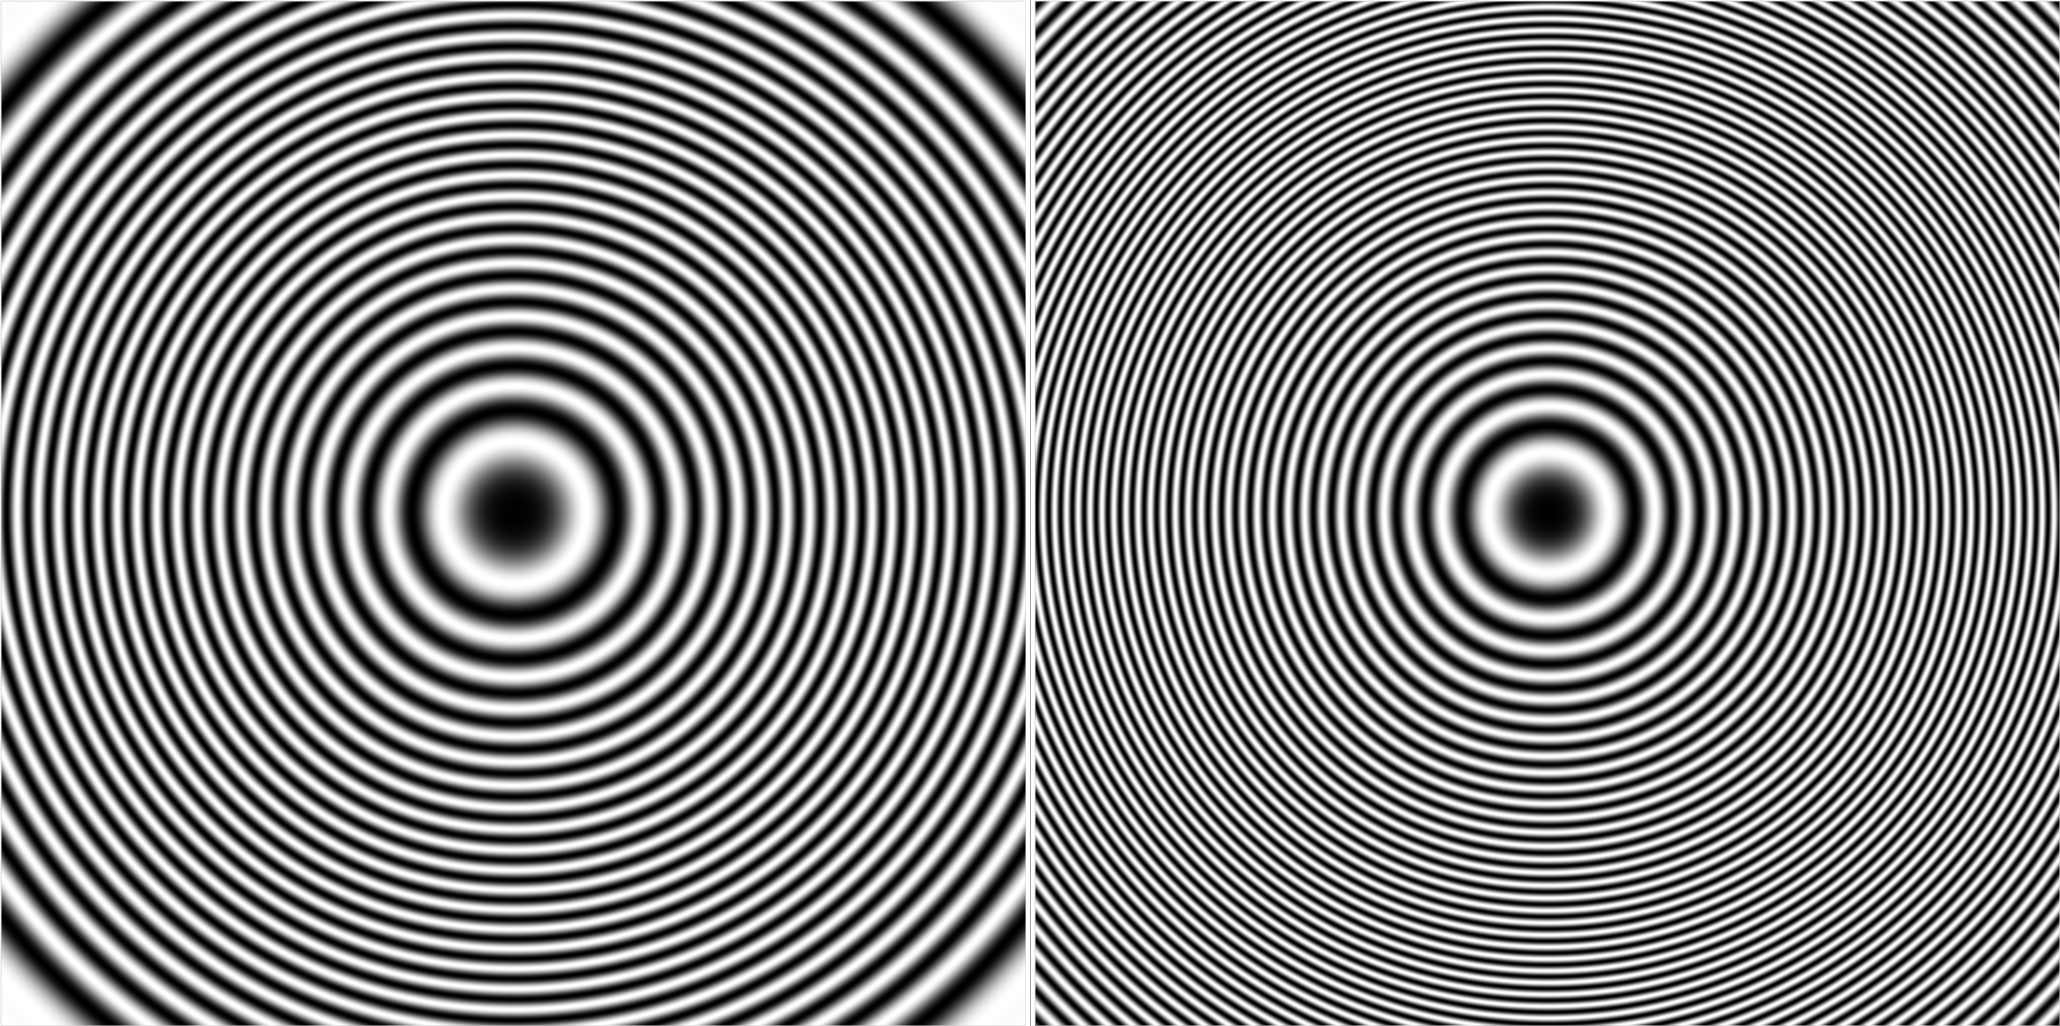
\includegraphics[width=\textwidth]{introduction/ctf_defocus_2d.png}
        \caption{2D power spectrum ($CTF^2$).}
        \label{fig:em_ctf_defocus_2d}
    \end{subfigure}%

    \begin{subfigure}{\textwidth}
        \centering
        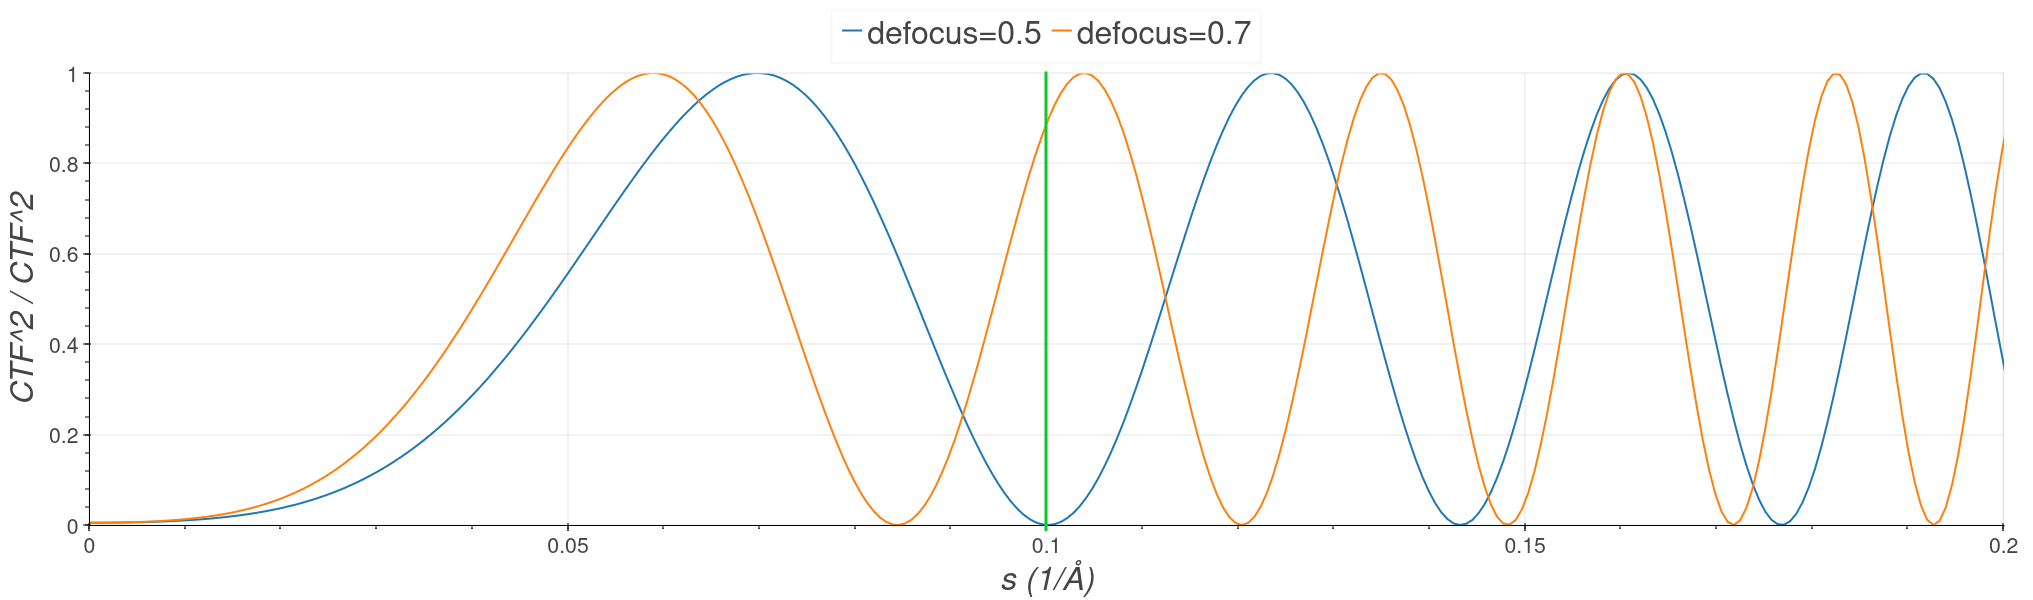
\includegraphics[width=\textwidth]{introduction/ctf_defocus_1d.png}
        \caption{1D rotational average.}
        \label{fig:em_ctf_defocus_1d}
    \end{subfigure}%

    \titledcaption[CTF: effect of defocus]{Simulated CTF of two images at different defoci. \textbf{(a)} 2D power spectrum ($CTF^2$). \textbf{(b)} 1D rotational average, highlighting in green the spatial frequency of 0.1 Å$^{-1}$, where the blue line (CTF at defocus 0.5 μm) is close to 0, whereas the orange line (CTF at defocus 0.7 μm) is close to 1. Images generated with: \url{https://ctfsimulation.streamlit.app/}~\cite{jiangWebbasedSimulationContrast2001}.}
    % https://ctfsimulation.streamlit.app/?ctf_type=CTF%5E2&ctf_type=CTF%5E2&defocus=0.5&defocus=0.7&over_sample=6&over_sample=6&share_url=1&show_2d=1
    \label{fig:em_ctf_defocus}
\end{figure}

To ensure all spatial frequencies are sampled, a data collection must include many images collected at a range of different defoci.

Of note is that since the CTF starts at 0, low spatial frequencies are always dampened; in pratical terms, this results in images where low resolution features (such as membranes and big objects) are harder to see, making it harder to distinguish objects from the noise, pick particles (\fullref{em_particle_picking}) and do further processing.
For this reason, a certain amount of defocus is always used, unfortunately at the cost of jumbling up the high frequency information with more CTF oscillation.
Alternatively, a phase plate can be used to shift the phase of the electrons by 90° and acquire images on focus (\autoref{fig:em_ctf_phase_shift}).
While phase plates are in theory the ideal solution to this problem, there are still some engineering and physical limitations that limit their use; several groups are currently working to overcome such hurdles~\cite{danevExpandingBoundariesCryoEM2017,schwartzLaserPhasePlate2019}.

\begin{figure}[ht]
    \centering
    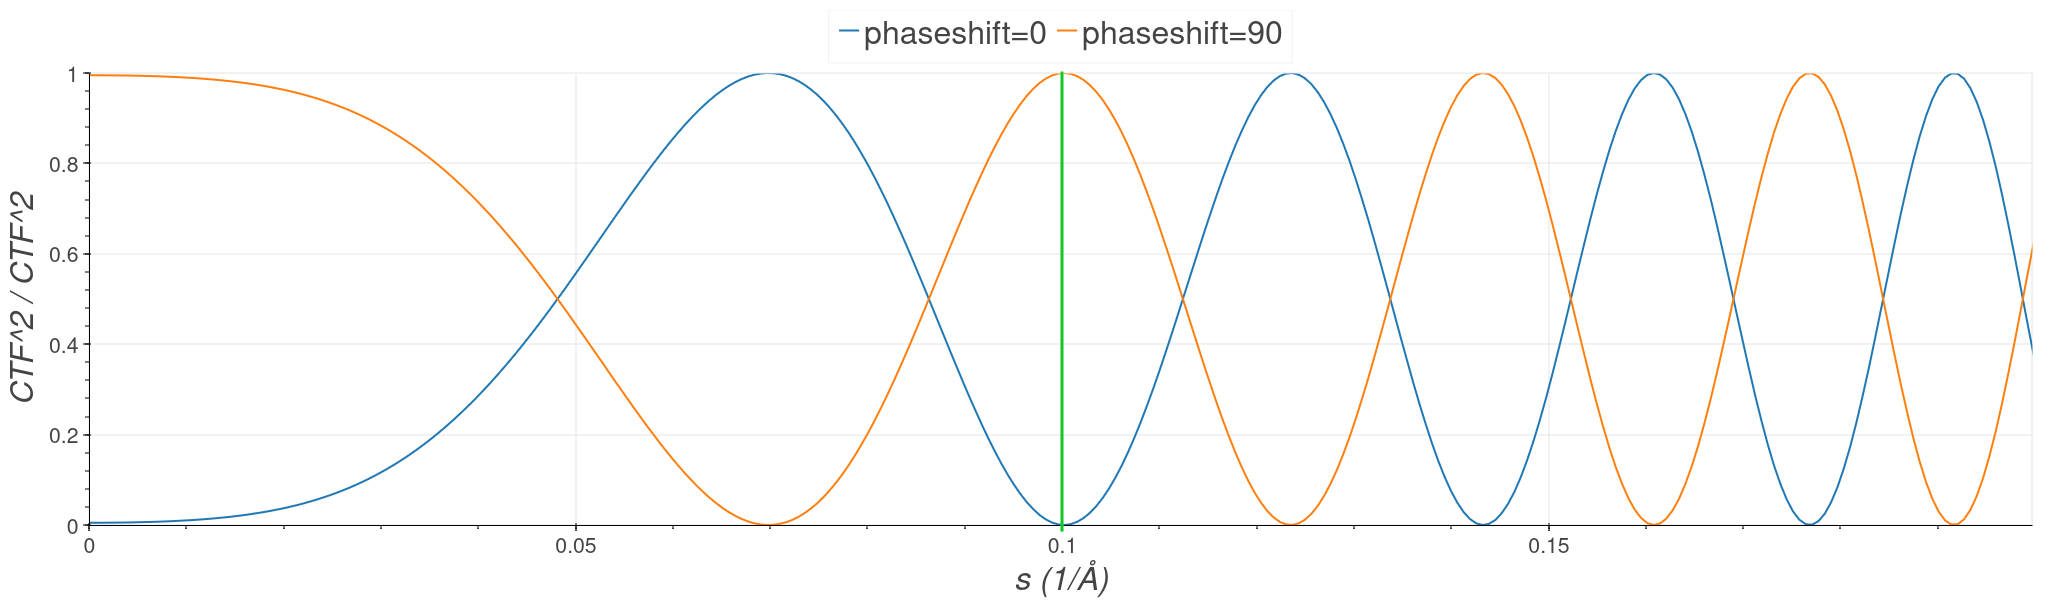
\includegraphics[width=\textwidth]{introduction/ctf_phase_shift.png}
    \titledcaption[CTF: effect of phase shift]{1D rotational average of a simulated CTF of two images at different phase shifts. Note how the phase-shifted CTF (orange) has a peak at spatial fequency 0, boosting low-resolution features. Image generated with: \url{https://ctfsimulation.streamlit.app/}~\cite{jiangWebbasedSimulationContrast2001}.}
    % https://ctfsimulation.streamlit.app/?ctf_type=CTF%5E2&ctf_type=CTF%5E2&defocus=0.5&defocus=0.7&over_sample=6&over_sample=6&share_url=1&show_2d=1&phaseshift=0.0&phaseshift=90.0
    \label{fig:em_ctf_phase_shift}
\end{figure}

The second component of the CTF is broadly called "envelope function", a dampening effect which attenuates the signal at higher resolutions.
It depends on many factors, such as lens aberrations, limitations of the electron gun, frame alignment imprecision, etc.
This effect is visible in the PS as an attenuation of the signal at higher resolutions (\autoref{fig:em_ctf_envelope}).
Since the PS (what we actually measure) is equivalent to the $CTF^2$, the dampening is exacerbated because values closer to 0 become even smaller and harder to detect.
Importantly, this effect is worse at higher defocus, contributing the worse high-resolution information transfer of higher defocus images.

\begin{figure}[ht]
    \centering
    \begin{subfigure}[B]{.42\textwidth}
        \centering
        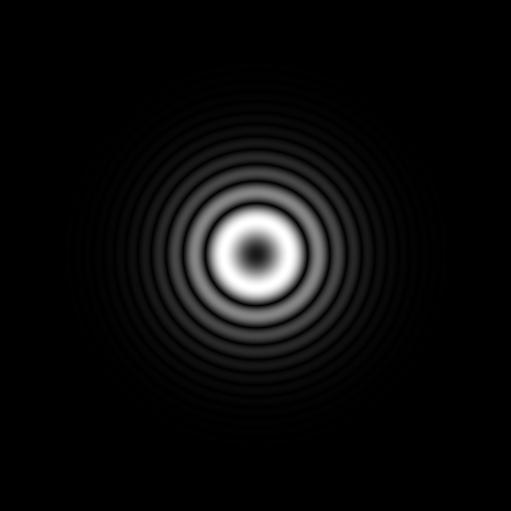
\includegraphics[width=\textwidth]{introduction/ctf_envelope_2d.png}
        \caption{2D power spectrum.}
        \label{fig:em_ctf_envelope_2d}
    \end{subfigure}%
    \hfill
    \begin{subfigure}[B]{.55\textwidth}
        \centering
        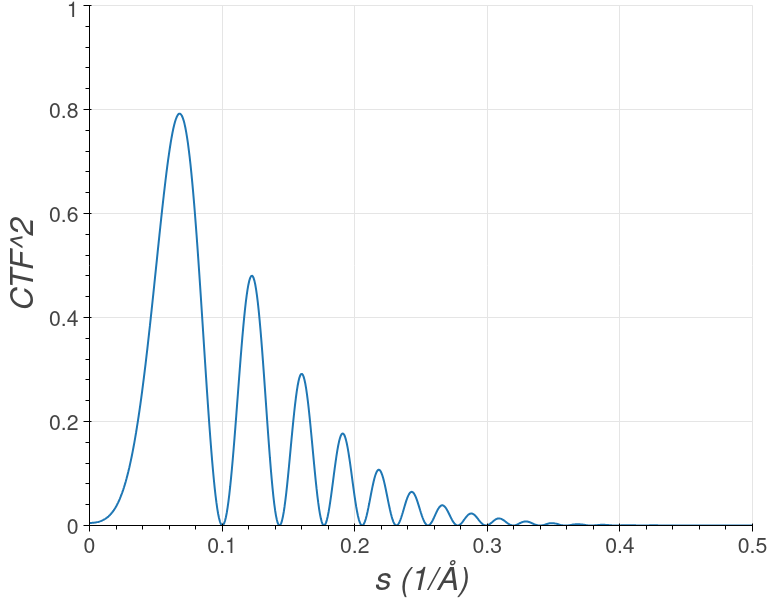
\includegraphics[width=\textwidth]{introduction/ctf_envelope_1d.png}
        \caption{1D rotational average.}
        \label{fig:em_ctf_envelope_1d}
    \end{subfigure}%
    \titledcaption[CTF: effect of the envelope function]{2D power spectrum (left) and 1D rotational average (right) of a simulated CTF, including some envelope function effects (such as beam convergence and energy spread). As a result, higher resolution frequencies are dampened, reducing the signal available for CTF estimation and high resolution reconstruction. Images generated with: \url{https://ctfsimulation.streamlit.app/}~\cite{jiangWebbasedSimulationContrast2001}.}
    % https://ctfsimulation.streamlit.app/?ctf_type=CTF%5E2&defocus=0.5&defocus=0.7&over_sample=3&share_url=1&show_2d=1&phaseshift=0.0&phaseshift=90.0&bfactor=10.0&alpha=0.3&dE=2.0&dI=7.0&dZ=0.1&dXY=0.1
    \label{fig:em_ctf_envelope}
\end{figure}

This signal decay, combined with the low SNR of the images, poses a resolution limit beyond which it is impossible to estimate (and therefore correct) the effect of the CTF on the image.

So far we discussed what happens to the fourier transform or PS of an image, that is in \textbf{fourier space}; in practice, the CTF has visible effects also in \textbf{real space}.
The signal becomes delocalized, blurring the image; as explained by the convolution theorem~\cite{wikipediaConvolutionTheorem2024}, this delocalization is the result of the convolution of the fourier transform of the CTF (known as Point Spread Function or PSF) with the image.
Delocalization of signal directly affects how image processing is performed; for example, particle picking should account for it by extracting bigger image patches to ensure delocalized signal can be deconvolved when CTF correcting (\fullref{em_particle_picking}).

\section{Preprocessing}\label{em_preprocessing}

Before particle picking, classification, and 3D reconstruction can be performed, the collected data must undergo a few preprocessing steps.

First, each movie generated during data collection must be aligned and averaged.
In state of the art applications, this alignment is typically done not only on a full frame level, but also in a localized fashion, by aligning image patches or by describing the system with a smooth deformation field~\cite{zhengMotionCor2AnisotropicCorrection2017,punjaniCryoSPARCAlgorithmsRapid2017,tegunovRealtimeCryoelectronMicroscopy2019}.

In state of the art software, similarly to how motion correction is treated, defocus (and thus CTF) is estimated at a local level, accounting for variability in the positioning of the sample with respect to the detector.
The parameters thus obtained are later used to correct for the CTF during classification and reconstruction (\fullref{em_classification} and \fullref{em_reconstruction}).
Modern workflows also offer the ability to later refine the deformation parameters as part of the refinement process (\fullref{em_refinement}).

Both motion correction and CTF estimation --- as well as many other steps and techniques in image processing --- rely on the ability to quantify the similarity of two signals; this is typically done by calculating the cross-correlation (CC) of the images or signals.

\subsection{Cross-correlation}\label{em_cross_correlation}

The CC of two signals (such as two images) is a measure of how similar the two signals are at all possible relative shifts.
The CC function of two signals will be higher for signals that present more similar features, and have a peak at the relative shift where the signals present strongest similarity (\autoref{fig:em_cross_correlation}).
This is a useful feature for most applications, because we often care about where exactly the similarity is high (e.g. for motion correction, particle picking and alignment (\fullref{em_particle_picking})).

\begin{figure}[ht]
    \centering
    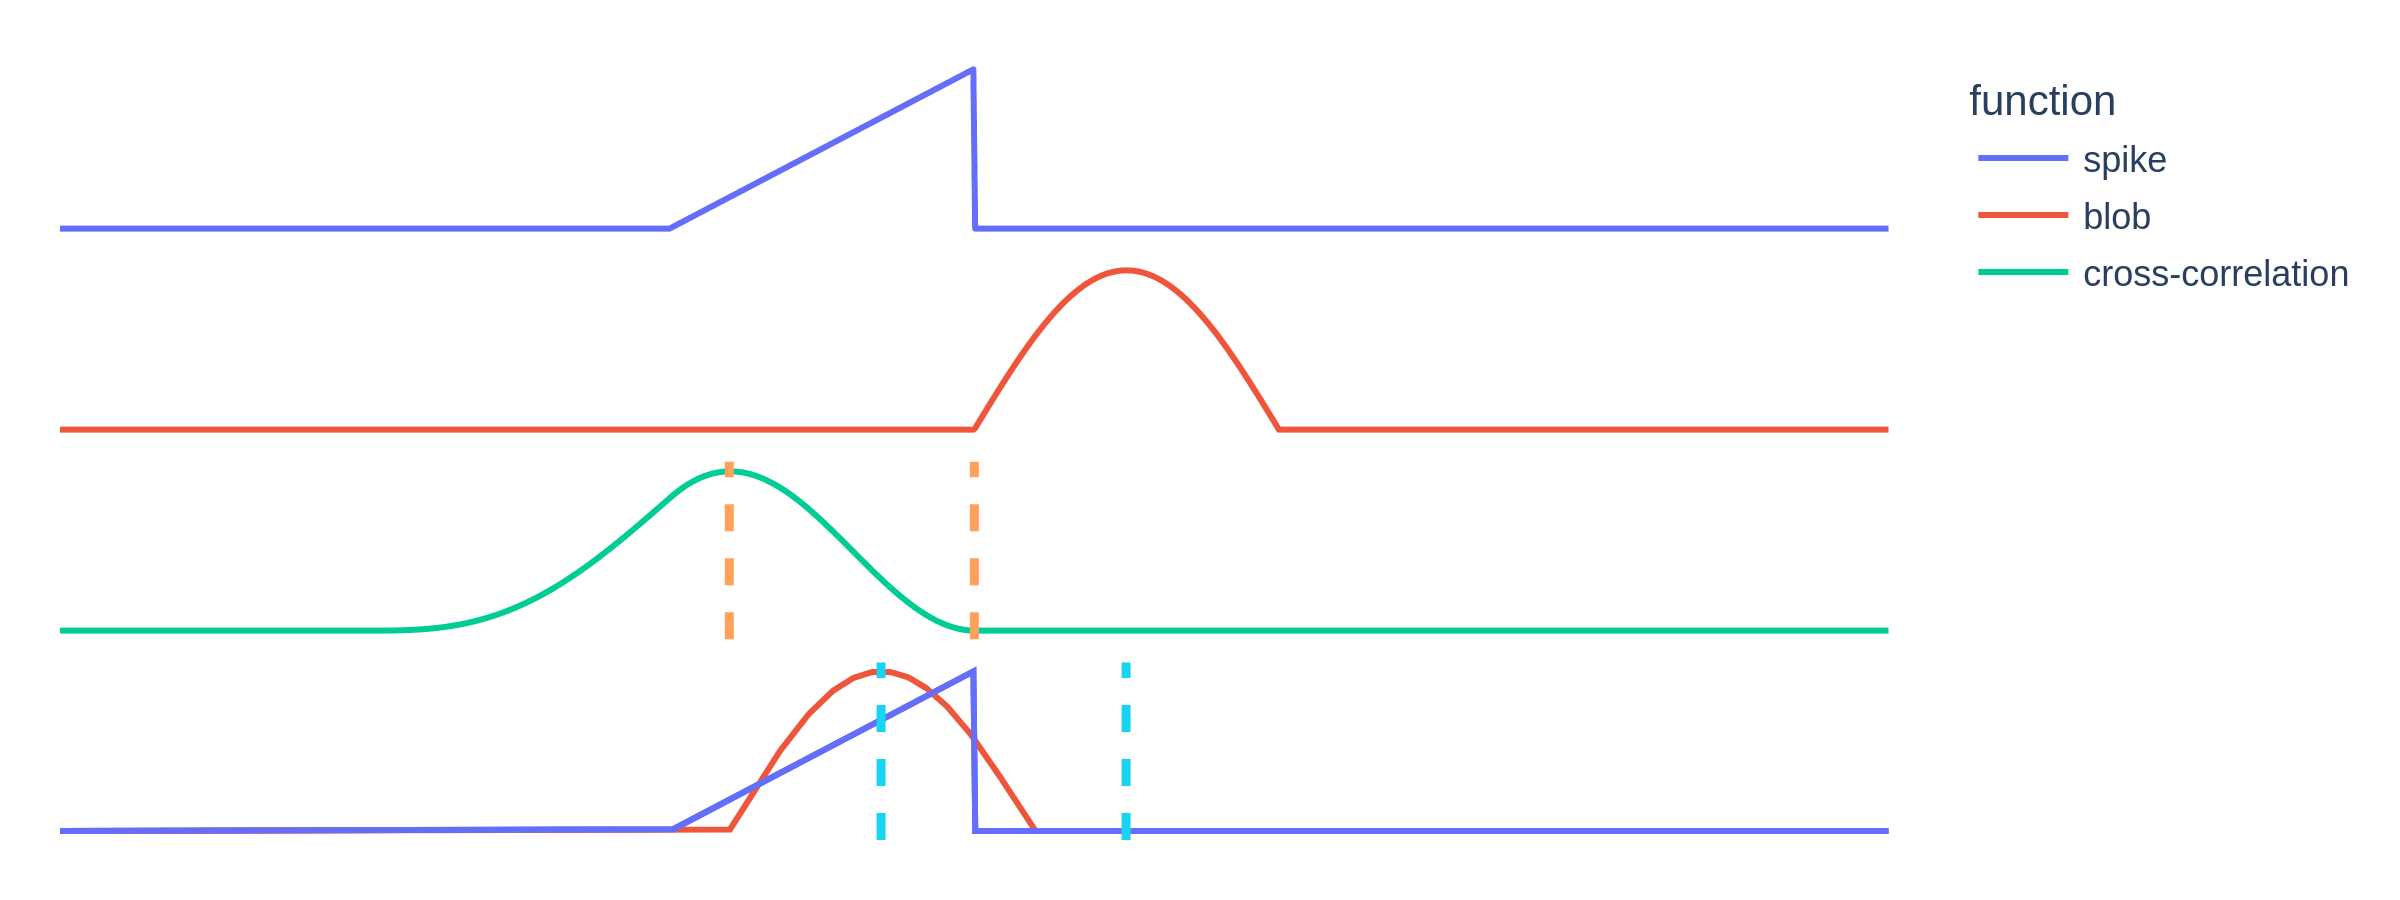
\includegraphics[width=\textwidth]{introduction/cross_correlation.png}
    \titledcaption[Cross-correlation of 1D signals]{Cross-correlation of two 1D signals, \texttt{spike} and \texttt{blob}. The position of the peak of the resulting \texttt{cross-correlation} indicates relative shift at which \texttt{blob} presents maximal similarity with \texttt{spike}. Shifting \texttt{blob} by the same amount shows the best overlap between the two signals.}
    \label{fig:em_cross_correlation}
    % TODO: generated with cc_image.py script. Should add somehow to thesis!
\end{figure}

In the case of 2D data, calculating the cross-correlation of two images often also includes the additional step of a rotational search, to account for the different in-plane rotation of particles that would otherwise be missed by simple CC.

\subsection{Filtering and denoising}\label{em_filtering_and_denoising}

Due to the low SNR of cryo-EM data, even motion-corrected micrographs can be surprisingly hard to interpret.
To enhance the contrast of biological features and better judge the quality of the data --- as well as improve the ability to distinguish particles from the background and from one another for the purposes of picking (\fullref{em_particle_picking}) --- micrographs often undergo a round of filtering and/or denoising.

The simplest --- and most commonly used --- type of filtering is fourier masking; by reducing or zeroing the values inside a disc or annulus in fourier space, the respective spatial frequencies are dampened in the image.
In practice, this is often used to remove high-frequency components (low-pass filter), but there are also sometimes benefits to the removal of other ranges of spatial frequencies (\autoref{fig:em_filtering}).

\begin{figure}[ht]
    \centering
    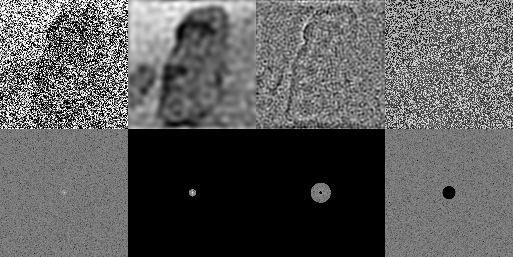
\includegraphics[width=\textwidth]{introduction/filtering.png}
    \titledcaption[Fourier filtering]{Examples of how filtering a noisy image (top left image) with different kinds of fourier masks (bottom row) produces different results (top row). From left to right: no filtering, low-pass, band-pass, high-pass. Low-pass filtering can restore interpretability of highly noisy images. As highlighted by the difference between the low-passed (second column) and high-passed (last column) images, a very small range of low spatial frequencies is actually responsible for the majority of our perception of the general shape of an object. Noise, on the other hand, more strongly affects high resolution information.}
    \label{fig:em_filtering}
    % TODO: made with filter.py
\end{figure}

In the last few years, denoising using ML tools has become standard practice, with algorithms such as noise2noise and noise2void~\cite{lehtinenNoise2NoiseLearningImage2018,krullNoise2VoidLearningDenoising2019} being implemented in several cryo-EM software suites~\cite{beplerTopazDenoiseGeneralDeep2020,tegunovRealtimeCryoelectronMicroscopy2019,buchholzCryoCAREContentAwareImage2018}.

\subsection{Dataset cleaning}
The dataset often contains bad images for various reasons: bad CTF estimation, too high motion, issues with autofocus, too thick or cracked ice, etc.
During preprocessing, these micrographs are usually discarded, either manually or by using batch automated tools which estimate the data quality.

Once the data is clean, motion corrected and CTF-estimated, the particles of interest can be picked for further processing.

\section{Particle picking}\label{em_particle_picking}
In order to reconstruct the 3D map of particles of interest, one first needs to locate them on the micrograph.
This procedure is called particle picking, and can be performed with varying levels of automation, and using several different techniques.
The most commonly used are variations of: manual picking, template matching, and ML tools.

Manual picking is generally more intuitive and can be very precise, but is also tedious and time-consuming.
Data may also be too noisy for humans to distinguish particles from one another and from the background, leading to missed particles or wrong picks.
To aid with manual picking, preprocessed micrographs are often filtered and denoised to improve the contrast (\fullref{em_filtering_and_denoising}).

To improve the picking speed and precision, template matching is often used to automate searching for a recognizable object.
This picking method requires a template, a small image of a 2D projection of the object of interest.
This can be obtained in a few ways: synthetically (by using a generated shape), by projecting a known map or model from previous work, or by using the results of a first round of 2D classification (\fullref{em_classification}) from a preliminary manual picking.
While the exact details of the algorithm may vary, at its core template matching relies on calculating the CC (\fullref{em_cross_correlation}) function between the template and the micrographs in order to locate putative particles positions in the whole dataset.

More recently, template matching is often being replaced with machine learning, which serves a similar purpose but can have a more nuanced understanding of surrounding context which helps reduce the false negatives and positives that are intrinsically present with template matching of noisy data.

There are also "structured" variants of all these picking methods, where some existing geometric and structural knowledge about the system is used to inform the picking in some way.
For example, filament picking is quite commonly used due to how widespread helical assemblies are in biology; it can be done manually~\cite{scheresRELIONImplementationBayesian2012,heHelicalReconstructionRELION2017}, with template-based methods~\cite{punjaniCryoSPARCAlgorithmsRapid2017}, and using ML~\cite{wagnerSPHIREcrYOLOFastAccurate2019,wagnerEvolutionSPHIREcrYOLOParticle2020}.

Regardless of the picking method, it is important to ensure that the target object is represented with projections from many different orientations; this will be crucial to properly reconstruct a 3D map of the object (\fullref{em_reconstruction}).

\section{2D classification}\label{em_classification}

Even with the best data and most advanced methods, picked particles typically contain a variety of several different objects, conformations, and spurious background or contamination picks; before moving on to reconstruction, the wheat should be separated from the chaff.
To do so, particles are split into groups based on similarity, in a process called 2D classification.

Once again, some form of cross-correlation (\fullref{em_cross_correlation}) is involved in the process, since the goal is to cluster together similar particles and separate different ones.
The algorithm is typically iterative: after generating an initial set of classes by averaging random particles, particle poses are progressively refined to find the best CC score.
Based on this score, each particle is assigned to a class (or a score for each class, in probabilistic models~\cite{scheresRELIONImplementationBayesian2012}), and for each class a class average is computed, combining the signal from all the particles belonging to that class. The more poses are refined, the more the signal that's shared by similar particles is boosted, improving the SRN of the class average.
Class averages are used to calculate the CC at each iteration, and used at the end of the process to inspect the dataset and select only the useful particles.

With this information, particle classes can be split into groups for further processing or discarded.
This is typically done manually by inspecting class averages and assigning each class to a group, depending on the goals of the project and the following processing steps.
For a uniform purified dataset, classification might only serve the purpose of discarding spurious picks.
For trickier samples (protein complexes, high conformational variability, non-uniform orientation distribution, cell-extract cryo-EM~\cite{suBuildRetrieveMethodology2021,kyrilisIntegrativeBiologyNative2019}), multiple groupings and several rounds of classification may be necessary to isolate each relevant state.

Once reasonably sure that each group contains only particles representing projections of different orientations of copies of the same object the 3D map of this object can be reconstructed --- though conformational variability might still be present and will need to be dealt with at a later stage.

\section{3D reconstruction}\label{em_reconstruction}

3D reconstruction is the process by which a volumetric map of an object can be reconstructed from 2D projections.
This is possible thanks to the central slice theorem~\cite{wikipediaProjectionsliceTheorem2023}, which provides a bidirectional mathematical relationship between a volume and its projections.

The theorem states that the fourier transform of the 2D projection of a volume at a certain orientation, is equal to the central slice through the fourier transform of the volume at the orientation perpendicular to the projection (\autoref{fig:em_central_slice}, panel A).

It's worth noting that the algorithms used by reconstruction software, while based on this principle, are often in practice not based on fourier-domain reconstruction, but use different methods such as weighted back-projection or iterative approaches like Simultaneous Algebraic Reconstruction Technique (SART) and Simultaneous Iterative Reconstruction Technique (SIRT)~\cite{andersenSimultaneousAlgebraicReconstruction1984,agulleiroFastTomographicReconstruction2011,wikipediaTomographicReconstruction2024}.

\begin{figure}[ht]
    \centering
    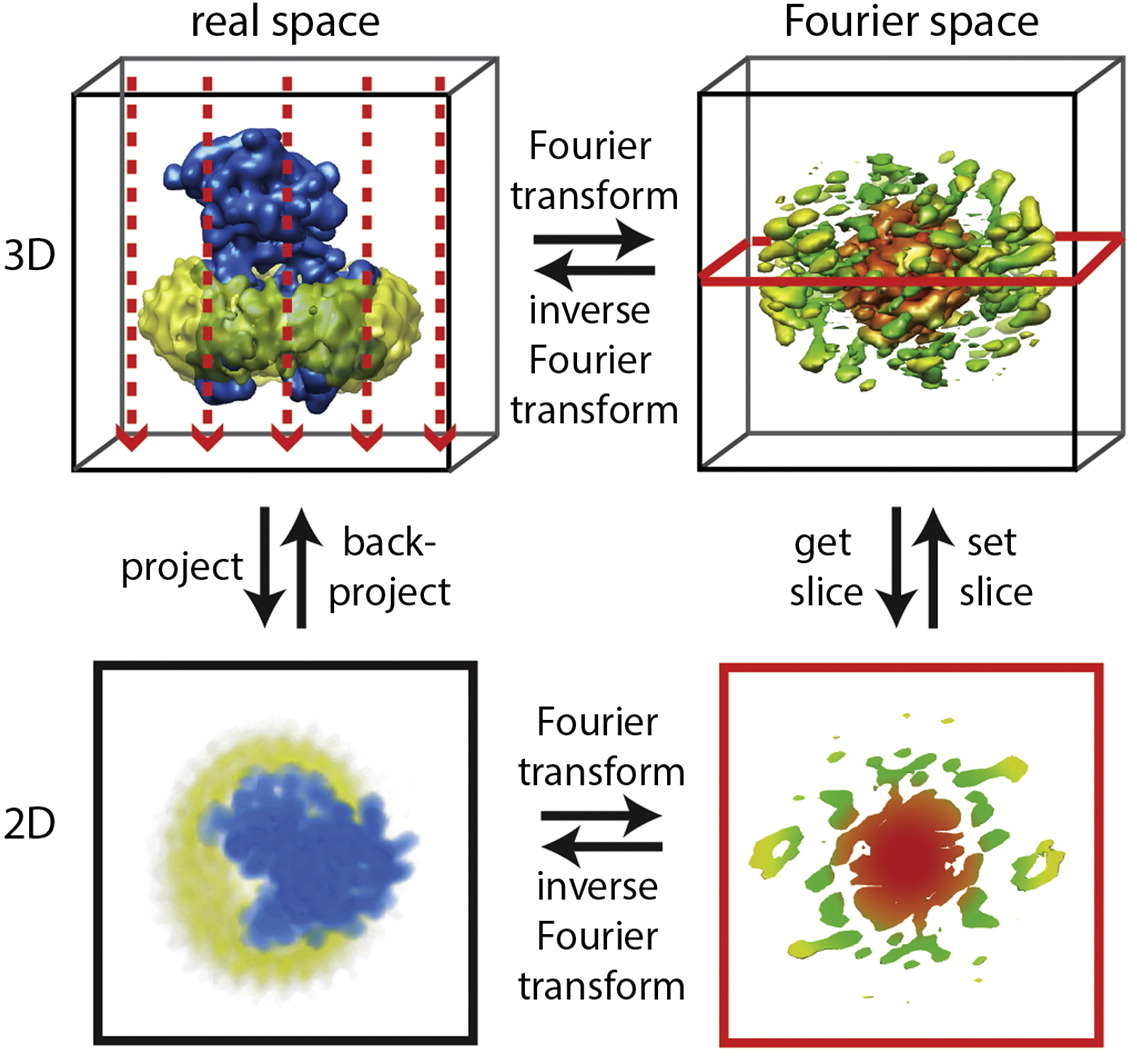
\includegraphics[width=.7\textwidth]{introduction/central_slice_theorem.png}
    \titledcaption[Central slice theorem]{Showcase of how the central slice theorem is used for 3D reconstruction in cryo-EM. \textbf{A.} A 2D projection of a 3D volume in real space at a certain orientation is equivalent to the 2D slice perpendicular to that orientation in fourier space. \textbf{B.} \textbf{C.} \textbf{D.} \textbf{E.}. Figure adapted from \citet{nogalesCryoEMUniqueTool2015}.}
    \label{fig:em_central_slice}
    % generated with fsc.py
\end{figure}

In the case of SPA, the central slice theorem allows us to combine the projection of many different particles, under the assumption that they come from near-identical copies of the same object.

It is crucial in this process that as many different orientations as possible are represented in the dataset.
This is because, in order to have an isotropically well-resolved reconstruction, we need to fill the 3D fourier space as much as possible with differently oriented central slices.

Similarly to 2D classification, 3D reconstruction is an iterative process where each particle is correlated to templates to find the best match.
This time, however, the templates are obtained by projecting a 3D model at different orientations, in a process called projection matching (\autoref{fig:em_projection_matching}).
Instead of assigning classes, projection matching refines the relative (3D) orientations of each particle relative to the original 3D object.
The 3D model is initally either derived from previous work, or generated \textit{ab initio} from the particles themselves.
During each iteration, particles' FTs are used to fill a 3D FT according to central slice theorem, which allows to generate a new 3D model.
The assigned orientations are progressively refined in order to improve the model resolution.
Once there is no longer significant improvement (\fullref{em_fsc}), the process stops, and the final 3D map is generated.

\begin{figure}[ht]
    \centering
    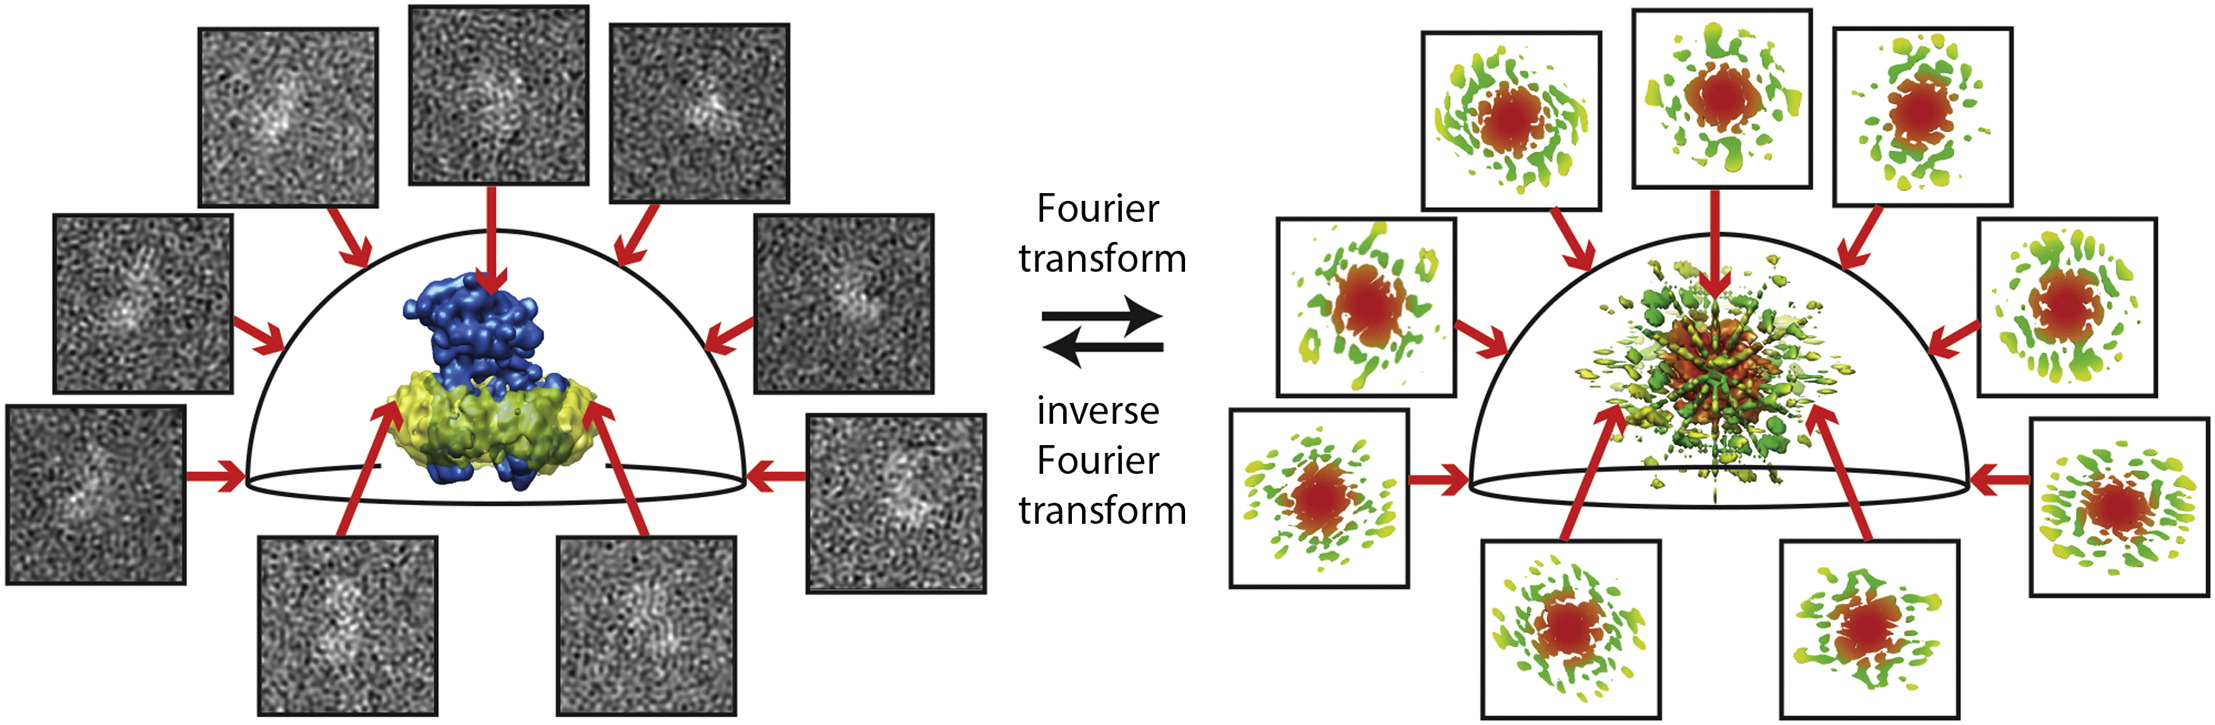
\includegraphics[width=\textwidth]{introduction/projection_matching.png}
    \titledcaption[Projection matching]{Projection matching in cryo-EM. Particle picks are assigned progressively better orientations that most closely match synthetic 2D projections generated from the current 3D model. By inserting the FT of each particle at the assigned orientation into the 3D fourier space, and then doing the inverse fourier transform to go back to real space, a new updated model is generated. Figure adapted from \citet{nogalesCryoEMUniqueTool2015}.}
    \label{fig:em_projection_matching}
\end{figure}

In some cases, it might be useful to go one step further and do 3D classification; this is essentially the same procedure, but using multiple 3D models at the same time to not only assign orientations, but also split particles into different classes.
This may be useful --- especially combined with some kind of mask to isolate areas of interest --- in cases where 2D classification was unable to separate out very similar objects.

When classification is too categorical to capture nuanced systems (such as continuous conformational ensembles), other kinds of procedures able to capture more variability may be used, such as principal component analysis (PCA)~\cite{castano-diezDynamoFlexibleUserfriendly2012,punjani3DVariabilityAnalysis2021}, multibody refinement~\cite{nakaneMultibodyRefinementCryoEM2021}, 3D flexible refinement~\cite{punjani3DFlexibleRefinement2022}, etc.

\subsection{FSC and gold standard}\label{em_fsc}
For most procedures that attempt to refine parameters in order to improve a 3D classification or reconstruction, a method is needed to estimate the quality (resolution) of the current model.

The established approach is called \textbf{gold standard} and relies on calculating the fourier shell correlation (FSC) of two independent halves of the data.
At the cost of halving the amount of data we can use at once to make a map, we gain the ability to estimate how trustworthy our reconstruction is.

At the beginning of the process, the dataset (which in the case of 3D reconstruction is the ensemble of picked particles) is randomly split in two halves.
At each iteration of the refinement, each half is used to generate an independent 3D reconstruction.
The fourier transforms of the two maps are then cross-correlated as a function of spatial frequency, giving a plot such as the one in \autoref{fig:em_fsc}.
A high correlation between fourier shell at the same spatial frequency indicates a high degree of reproducibility of those frequency components: that is, up to that resolution, the map can be trusted.
The threshold typically used to formally determine the "resolution of the map" is 0.143, for both mathematical and historical reasons related to the interpretability of X-ray crystallography maps~\cite{rosenthalOptimalDeterminationParticle2003}.

\begin{figure}[ht]
    \centering
    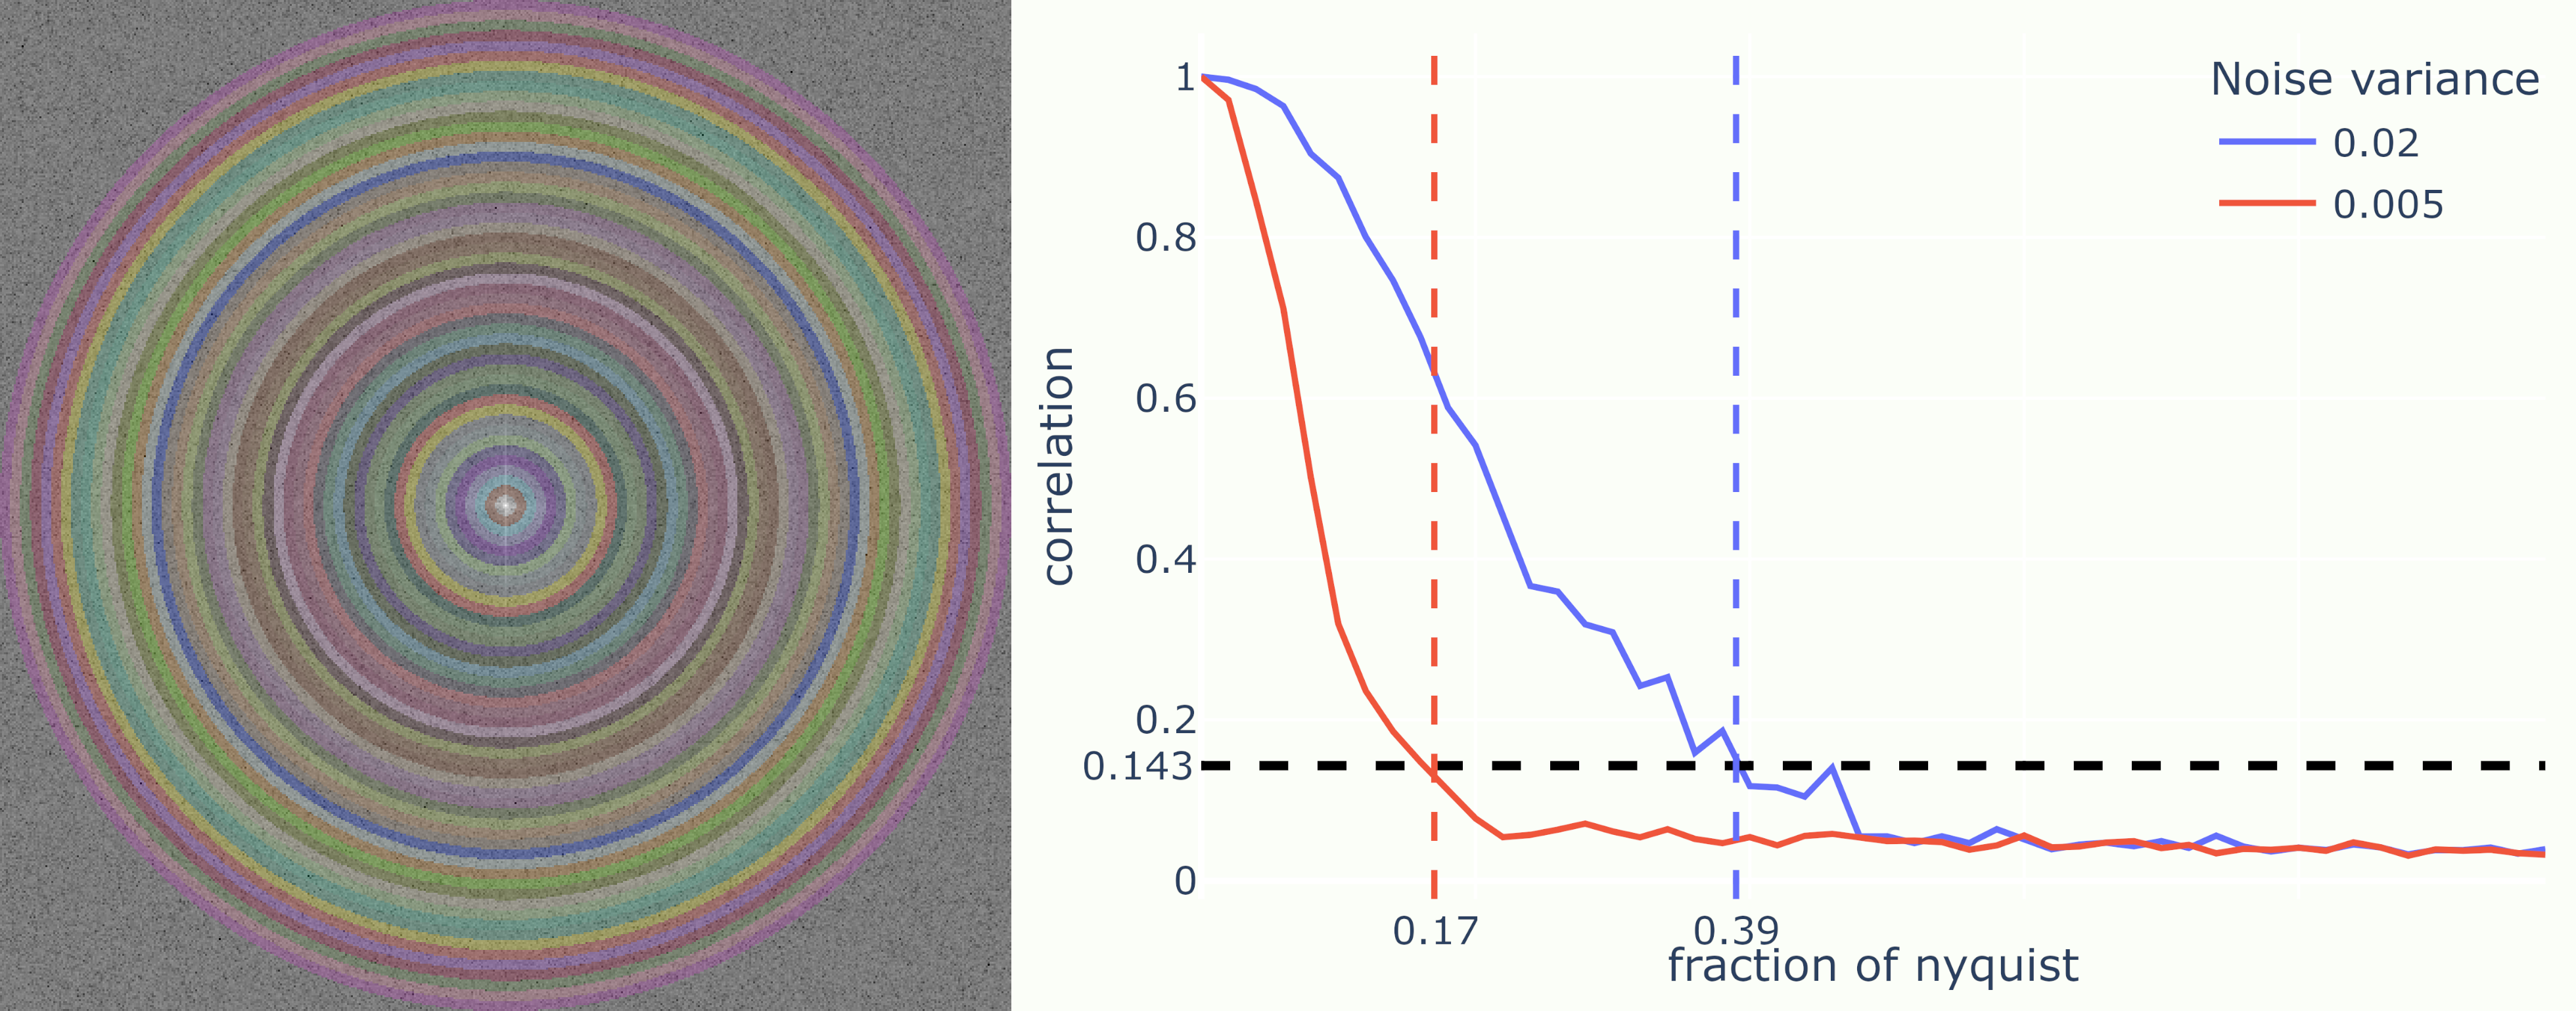
\includegraphics[width=\textwidth]{introduction/fsc.png}
    \titledcaption[Fourier shell correlation]{Showcase of a 2D version of fourier shell correlation. Gaussian noise was applied to two identical images, which were then compared by gradually cross-correlating concentric shells (left). The resulting plot (right) is a measure of the similarity as a function of spatial frequency. As spatial frequency increases, noise becomes dominant, degrading correlation and thus the trustworthiness of the data. The threshold of 0.143 is used to determine the final resolution, which is higher for the less noisy image.}
    \label{fig:em_fsc}
    % TODO: made with script fsc.py
\end{figure}

\subsection{Map post-processing}
Reconstructed maps are normally post-processed to improve interpretability and usability in model building procedures.

Different types of masking, filtering, and denoising can be applied, depending on the downstream steps.

% TODO: feels like I should expand, but it's also not very important here. Sharpening?

\section{Refinement}\label{em_refinement}
Once a 3D model is obtained, several state of the art software pipelines offer the ability to refine previously-defined parameters.
The parameters that can be refined range from particle positions and orientations, to CTF estimation and motion correction, to more complex artifact-inducing factors such as lens aberrations and Ewald sphere curvature~\cite{tegunovMultiparticleCryoEMRefinement2021,punjaniCryoSPARCAlgorithmsRapid2017,scheresRELIONImplementationBayesian2012}.
While resolution of the resulting 3D reconstruction is the most obvious parameter used to validate the improvements, there are several other criteria that may be considered, such as local resolution, angular distribution of views, map continuity, etc.

The implementation details of refinement procedures are often quite different between software, but are generally based on an iterative process where parameters are adjusted on a per-particle basis, and a new 3D reconstruction is generated and validated via FSC to estimate the effects of the correction applied.

These procedures can have dramatic effects on the final resolution of a map, especially when pushing for sub-nanometer resolution where small aberrations and artifacts can have significant effects on the achievable resolution.

\section{Model building}

If a map reaches high enough resolution, it is possible to build an atomic model based on the volume density.
This process is called model building, and is typically done with a mix of manual and automated tools.

Models are built by placing amino acids (or other structural components) so that their electron occupancy matches the density map obtained from 3D reconstruction.
Some recent tools manage to fully automate this process for maps of high enough resolution (\lesssim4 Å), even without knowing the protein's sequence~\cite{jamaliAutomatedModelBuilding2024}.
